\section{Boundary data and a common interior region}
\label{data:section}

We first convert the measurements into data that can be continued in the
interior. Equality of the energy maps determines the full boundary jets
on the measured patch. These jets allow us to attach the same exterior
cap to both metrics. Sources in that cap then supply common Green data
and the finite families of harmonic functions needed in the local proof.

We use $\Delta_g=\operatorname{div}_g\nabla_g$ and positive Riemannian
densities throughout. In particular, no orientation is chosen.
The Dirichlet realization of $L_g=-\Delta_g$ on a compact connected
smooth manifold with nonempty boundary is invertible: its quadratic
form on $H^1_0$ is coercive. Smooth sources and boundary values give
solutions smooth up to the boundary. We use interior elliptic
regularity and unique continuation for smooth scalar second-order
elliptic operators with real positive principal part, including a
metric Laplacian multiplied by a positive smooth function.
Here unique continuation means that an existing
solution which vanishes on a nonempty open subset of a connected
domain vanishes throughout that domain; see
\citep[Theorem~8]{KochTataru2005}.
For a positive scalar elliptic principal symbol, the local
noncharacteristic-surface condition applies at every smooth
hypersurface; propagation through overlapping coordinate balls gives
this open-set form of continuation.

We will also use its boundary version. If a smooth harmonic function
has both zero value and zero normal derivative on an open boundary
patch, extend the metric smoothly across that patch and the function
by zero. Green's formula shows that the extended function solves the
equation distributionally: neither a value jump nor a flux jump
remains. Elliptic regularity and interior unique continuation give
vanishing in a neighborhood of the patch, and then in the connected
interior.

\subsection{The density and the boundary jets}

The distinction between the measured energy operator and the ordinary
unit-normal DN operator matters in the first step. The latter sends
$f$ to $\partial_{\nu_g}u_f$; the former sends it to the density
$\partial_{\nu_g}u_f\,dS_g$.

\begin{lemma}[Boundary jets]\label{data:jets}
Let $g_1,g_2$ be smooth metrics on a compact connected smooth
$n$-manifold $M$ with nonempty boundary, where $n\ge3$. Suppose their
energy maps agree for inputs and observations in a nonempty relatively
open set $\Gamma\subset\partial M$. In boundary-normal coordinates
for the respective metrics, based on the same coordinates on
$\Gamma$, their complete boundary Taylor jets agree.
\end{lemma}

\begin{proof}
Fix a boundary chart compactly contained in $\Gamma$, write
$m=n-1\ge2$, and let $h$ denote the tangential metric matrix.
Relative to the coordinate density, the energy operator has principal
symbol
\[
 e_1(z,\xi)=\sqrt{\det h(z)}
             \sqrt{h^{ab}(z)\xi_a\xi_b}.
\]
Thus its square determines the positive matrix
\[
 C=(\det h)h^{-1},\qquad
 \det C=(\det h)^{m-1},\qquad
 h=(\det C)^{1/(m-1)}C^{-1}.
\]
The two induced metrics, and hence their boundary densities, are
therefore equal. Dividing the common density-valued operator by this
known density gives equality of the ordinary DN operators locally.
Cutoffs supported in $\Gamma$ and equal to one near a chosen point
give equality of their complete symbols there.

We give the scalar symbol recursion to make its smooth and local
content explicit. This boundary determination goes back to
\citet{LeeUhlmann1989}; see also
\citet[Theorem~1.1(ii) and Proposition~3.1]{JoshiLionheart2005}.
In inward normal coordinates $s\ge0$, write
\[
 g=ds^2+h(s,z),\qquad
 a=\frac12\tr(h^{-1}\partial_s h),\qquad
 L_g=-\partial_s^2-a\partial_s+P,
\]
where $P=-\Delta_{h(s)}$ is tangential. Smooth boundary factorization
gives a tangential operator $B(s)$ of order one, with positive
principal symbol, such that
\begin{equation}\label{data:factorization}
 L_g=(-\partial_s+B-a)(\partial_s+B)
          \pmod{\Psi^{-\infty}},\qquad
 B^2-aB-\partial_sB=P\pmod{\Psi^{-\infty}}.
\end{equation}
Here the remainders are tangentially smoothing and depend smoothly on
$s$. The local Poisson parametrix identifies $B(0)$, modulo smoothing,
with the outward DN operator: the decaying branch satisfies
$(\partial_s+B)u=0$ and $\partial_\nu=-\partial_s$.
This is a local factorization for smooth coefficients; it makes no
analyticity assumption.

For precision, use left symbols and $D_z=-i\partial_z$, so
\[
 b\mathbin{\#}c\sim
 \sum_\alpha\frac{(1/i)^{|\alpha|}}{\alpha!}
       (\partial_\xi^\alpha b)(\partial_z^\alpha c).
\]
Write $b\sim b_1+b_0+b_{-1}+\cdots$ for the symbol of $B$ and
$p=p_2+p_1$ for that of $P$. Then
\[
 b_1=\rho=(h^{ab}\xi_a\xi_b)^{1/2},\qquad
 b\#b-ab-\partial_sb=p.
\]
The equation of degree one is
\[
 2\rho b_0+\frac1i\partial_\xi\rho\cdot\partial_z\rho
             -a\rho-\partial_s\rho=p_1.
\]
The terms $p_1$ and the tangential composition term involve only $h$
and its tangential derivatives. Since
\[
 \partial_s\rho
 =-\frac{(\partial_s h)(\xi^\sharp,\xi^\sharp)}{2\rho},
\]
the part of $b_0$ containing a normal derivative is
\[
 \frac14\left(\tr_h\partial_s h
       -\frac{(\partial_s h)(\xi^\sharp,\xi^\sharp)}{\rho^2}\right).
\]
At each subsequent degree the new coefficient is obtained from
\[
 2\rho b_{1-k}=\partial_s b_{2-k}+R_k,\qquad k\ge2,
\]
where $R_k$ uses normal derivatives of $h$ only through order $k-1$
and finitely many tangential derivatives. Indeed all other terms in
the symbol product use earlier coefficients, and tangential
differentiation does not increase normal derivative order.
Writing $A_k=\partial_s^k h$, induction gives the highest-jet term
\begin{equation}\label{data:highest-jet}
 b_{1-k}=
 \frac{1}{4(2\rho)^{k-1}}
 \left(\tr_h A_k-
        \frac{A_k(\xi^\sharp,\xi^\sharp)}{\rho^2}\right)
 +\text{terms involving lower normal jets}.
\end{equation}
Differentiating $\rho$, the raising of indices, or the coefficient
in the preceding induction step contributes only lower-jet terms.

Suppose the two normal jets agree through order $k-1$ as smooth
functions on the boundary chart. Their tangential derivatives also
agree. Equality of the symbols and Equation~\eqref{data:highest-jet}
give, for $A=\partial_s^k(h_1-h_2)|_{s=0}$,
\[
 \tr_h A-A(v,v)=0\qquad(|v|_h=1).
\]
Polarization yields $A=(\tr_h A)h$. Taking the trace gives
$(m-1)\tr_h A=0$, so $A=0$. Starting from the already recovered
boundary metric, induction proves all normal and mixed jet
equalities. The normal metric components are $g_{ss}=1$ and
$g_{sa}=0$, so these are the full metric jets.

Every step is local to a half-coordinate ball and uses densities.
Although the differential-form formulation in
\citep{JoshiLionheart2005} assumes orientability, this scalar
coordinate proof requires none. Other boundary components affect
only the local smoothing remainder. Finally, equality of smooth
jets asserts no equality in an interior collar.
\end{proof}

\subsection{Attaching a common cap}

The jets provide a common region on the exterior side of a smaller
patch. The following energy argument transfers the measured data to
that region without making assumptions on the inaccessible boundary.

\begin{proposition}[Common cap and Green data]\label{data:cap}
Under the hypotheses of Lemma~\ref{data:jets}, there are compact
connected smooth extensions $(M_j^e,g_j^e)$ of $(M,g_j)$ and an
identified connected open exterior cap $E$ on which the extended
metrics agree. The cap is attached through a nonempty open set
$P_0\Subset\Gamma$. The extended zero-Dirichlet Green kernels satisfy
\[
 G_1(x,y)=G_2(x,y),\qquad x,y\in E,\quad x\ne y.
\]
For every $F\in C_c^\infty(E)$, the two extended zero-Dirichlet
solutions with source $F$ agree on $E$.
\end{proposition}

\begin{proof}
Choose a boundary coordinate patch $P\Subset\Gamma$ and a
nonnegative smooth bump $b$ with $\supp b\Subset P$ and connected,
nonempty positivity set $P_0=\{b>0\}$. Use the separate inward
normal collars of Lemma~\ref{data:jets}, and replace the boundary
$s=0$ by the graph $s=-b(z)$. Take $b$ sufficiently small that this
graph lies in a collar. It gives smooth compact connected extended
manifolds. Their common open added part is
\[
 E=\{(z,s):-b(z)<s<0\}.
\]
Extend the first metric smoothly to negative $s$ and use the same
exterior metric for the second. A smooth extension of its coordinate
coefficients exists in a collar and remains positive definite after
shortening the collar. Their jets match on an open neighborhood of
$\supp b$. Pasting across the entire hypersurface $s=0$ in that
neighborhood is therefore smooth, to every order. Restricting this
pasting to $s\ge-b(z)$ proves smoothness also at the edges of the
bump. We henceforth omit the superscript on the extended metrics.

For the following comparison, identify the two extensions by the
identity on the original $M$ and by the common collar coordinates
on $E$. This identification and its inverse are smooth up to
each side of the seam, with bounded derivatives, and agree on the
seam. In collar charts they are therefore bi-Lipschitz. In particular
they identify the spaces $H^1_0$ on the two extensions.

Fix a real $F\in C_c^\infty(E)$ and let $w_j$ minimize
\[
 \mathcal J_j(w)=\frac12\int_{M_j^e}|dw|_{g_j}^2\,dV_{g_j}
                       -\int_E Fw\,dV_{g_j}
       \quad\text{on }H^1_0(M_j^e).
\]
The minimizers are smooth up to the extended boundary and solve
$-\Delta_{g_j}w_j=F$. Their traces $h_j$ on the original boundary
are smooth and supported in $\supp b\Subset\Gamma$: wherever
$b=0$, that boundary is also the new zero-data boundary.
Transport $w_1$ by this identification and replace it inside the
original manifold by the $g_2$-harmonic
extension of $h_1$, leaving it unchanged on $E$. The difference
between the replacement and the transported $w_1$ is the zero extension of a function
in $H^1_0(M)$; thus the replacement is an admissible competitor in
$H^1_0(M_2^e)$. This argument does not require the narrowing cap to
have a regular boundary at its edges.

The interior energies before and after replacement are the equal
quadratic energies of $h_1$ for the two measured maps. The cap metric
and source pairing are common. Hence
$\min\mathcal J_2\le\min\mathcal J_1$. Reversing the roles gives
equality. Strict convexity of the Dirichlet form makes the replacement
equal to $w_2$, proving $w_1=w_2$ on $E$.

Normalize the symmetric Dirichlet Green kernels by
\begin{equation}\label{data:green-normalization}
 -\Delta_{g_j,x}G_j(x,y)=\delta_y^{g_j}(x),\qquad
 G_j(\,\cdot\,,y)|_{\partial M_j^e}=0,
 \qquad
 w_j(x)=\int_{M_j^e}G_j(x,y)F(y)\,dV_{g_j}(y),
\end{equation}
where the point mass has unit mass relative to metric volume.
The source densities are identical on $E$. Varying $F$ gives
equality of the distribution kernels on $E\times E$, and therefore
pointwise equality off the diagonal.
\end{proof}

Fix a nonempty open source set $U_0\Subset E$.
Figure~\ref{data:cap-figure} shows the two boundaries and a possible
choice of this set.

\begin{figure}[htbp]
\centering
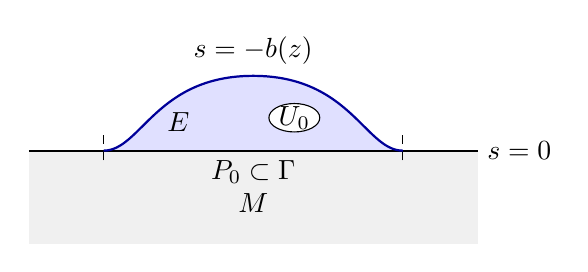
\begin{tikzpicture}[scale=0.95]
 \fill[gray!12] (-3,-1.25) rectangle (3,0);
 \fill[blue!12] (-2,0) .. controls (-1.5,0) and (-1.3,1.0) .. (0,1.0)
                 .. controls (1.3,1.0) and (1.5,0) .. (2,0) -- cycle;
 \draw[thick] (-3,0)--(3,0);
 \draw[thick,blue!60!black] (-2,0)
                 .. controls (-1.5,0) and (-1.3,1.0) .. (0,1.0)
                 .. controls (1.3,1.0) and (1.5,0) .. (2,0);
 \draw[dashed] (-2,-0.13)--(-2,0.23);
 \draw[dashed] (2,-0.13)--(2,0.23);
 \node at (0,-0.7) {$M$};
 \node at (-1,0.38) {$E$};
 \draw[fill=white] (0.55,0.44) ellipse (0.34 and 0.19);
 \node at (0.55,0.44) {$U_0$};
 \node[above] at (0,1.02) {$s=-b(z)$};
 \node[below] at (0,0) {$P_0\subset\Gamma$};
 \node[right] at (3,0) {$s=0$};
\end{tikzpicture}
\caption{A local schematic cross-section of the common exterior cap.
The boundary moves only over a compact subset of the measured patch.
The oval is a nonempty open source set $U_0$ with closure inside $E$.
The proof uses the smooth graph, including its flat bump edges.}
\label{data:cap-figure}
\end{figure}

\subsection{Harmonic tests from sources in the cap}

For $f\in C_c^\infty(U_0)$, let $u_f^j$ be the zero-Dirichlet solution
of $L_{g_j}u_f^j=f$ on $M_j^e$. Define its evaluation at a point by
\begin{equation}\label{data:evaluations}
 I_j(p)(f)=u_f^j(p).
\end{equation}
Equality of evaluations means equality for every such source $f$.
Proposition~\ref{data:cap} gives $I_1=I_2$ on $E$. The functions
$u_f^j$ are harmonic away from $\overline{U_0}$; we only use their
harmonic jets there.

This use of harmonic evaluations follows the Poisson and source
embedding approaches of \citet[Sections~2 and~6.1]{LLS20}.
The restricted-source approximation and separation results appear in
\citep[Appendix~A, Propositions~A.6--A.7]{LLS20}.
The point-distribution argument below has a close antecedent in
\citet[Chapter~III, Section~3, proof of Theorem~6]{Malgrange1956}:
unique continuation forces the inverse of an annihilating point
distribution to have point support, and differential order then
determines that distribution. We give the full argument for the
required second jets and positive densities.

\begin{lemma}[Separation and finite harmonic jets]\label{data:jet-family}
Let $(N,g)$ be a compact connected smooth manifold with nonempty
boundary and dimension $n\ge2$. Let $U\Subset N^\circ$ be
nonempty and open, and let $R=L_{g,D}^{-1}$. Then:
\begin{enumerate}[label=\textup{(\roman*)}]
 \item The functionals $I(p):f\mapsto Rf(p)$,
       $f\in C_c^\infty(U)$, separate distinct interior points.
       They are nonzero in the interior and zero on the boundary.
       For each fixed $f$, they depend continuously on $p\in N$.
 \item If $p\in N^\circ\setminus\overline U$, the second jets of
       $Rf$ at $p$ fill exactly the hyperplane defined by
       $L_g u(p)=0$. In particular they provide harmonic coordinates
       near $p$ and any finite spanning family of harmonic Hessians
       in those coordinates.
\end{enumerate}
\end{lemma}

\begin{proof}
Continuity and the zero boundary values follow from smooth Dirichlet
regularity. For a nonnegative nonzero $f\in C_c^\infty(U)$,
the maximum principle and its strong form give $Rf>0$ throughout
$N^\circ$. Thus the interior functionals are nonzero.

We prove the jet assertion by finite-dimensional duality. Let $T$
be a linear functional on second jets at $p$ annihilating all
$Rf$, represented as a distribution of order at most two supported
at $p$. Define $w=RT$ by transposition with the metric density.
The Dirichlet inverse is self-adjoint, so
\[
 \langle w,f\rangle=\langle T,Rf\rangle=0,
           \qquad f\in C_c^\infty(U).
\]
Thus $w=0$ on $U$ and $L_gw=T$. Away from $p$ it is smooth and
harmonic by elliptic regularity. The punctured interior is connected:
a path meeting $p$ can be diverted in a small punctured coordinate
ball, whose spheres are connected in dimension at least two.
Unique continuation consequently gives $\supp w\subset\{p\}$.

A distribution supported at one point is a finite sum
\[
 w=\sum_{|\alpha|\le k}c_\alpha\partial^\alpha\delta_p.
\]
If $w\ne0$ and $k$ is its highest derivative order, then $L_gw$
has exact order $k+2$. Indeed its highest coefficient polynomial
is the product of the nonzero degree-$k$ coefficient polynomial
and the nonzero elliptic quadratic principal symbol. Such a product
cannot vanish. Since $T$ has order at most two, $w=c\delta_p$.
Hence the annihilator consists precisely of multiples of
$u\mapsto L_gu(p)$. That functional does annihilate the source
solutions because $p\notin\overline U$. Finite-dimensional duality
proves that their jet range is the whole stated hyperplane.

To prove separation, suppose $I(p)=I(q)$ for distinct interior
points. Apply the same transposition argument to
$T=\delta_p-\delta_q$. The solution $RT$ vanishes on $U$,
and UCP on the connected interior with these two points removed
shows that it is supported at those points. The argument still
applies if a point lies in $U$, since the initial vanishing on $U$
is distributional. At each support point a nonzero point-supported
distribution has an elliptic image of order at least two.
It cannot have the order-zero image $\delta_p-\delta_q$.
This contradiction proves separation.

Finally the equation constraint allows arbitrary first derivatives,
by adjusting the Hessian. Choose $n$ source solutions with independent
differentials; their tuple is a harmonic coordinate chart. In this
chart the first-order coefficients of $\Delta_g$ vanish, so the
ordinary coordinate Hessians have precisely the constraint
$g^{ab}\partial_{ab}u=0$. The jet conclusion supplies a basis for
that hyperplane, with zero first derivatives if desired. A chosen
finite basis remains spanning, with a positive Gram bound, after
shrinking the chart.
\end{proof}

\begin{remark}\label{data:local-pairs}
At any point outside $\overline{U_0}$ we may use finitely many
pairs $(u_f^1,u_f^2)$ to supply the harmonic coordinates and Hessians
in the local argument. Once chosen, these functions remain fixed
while the spatial scales shrink. The constant pair $(1,1)$ is
adjoined separately; it is not a zero-boundary source solution.
All these statements are scalar and use positive densities, so
they retain nonorientable manifolds and arbitrary boundary components.
\end{remark}
